\documentclass[11pt]{article}
\usepackage{amsfonts,amsthm,amsmath,amssymb, hyperref, dsfont, enumitem, bbm}
\usepackage{array}
\usepackage{epsfig}
\usepackage{fullpage}
\usepackage{color}
\usepackage{epigraph}
\renewcommand{\epigraphflush}{center}
\usepackage[framemethod=tikz]{mdframed}
\usepackage{titlesec}
\usepackage{ellipsis}
\usepackage{subcaption}
\usepackage[normalem]{ulem}
\usepackage{todonotes}


\titleformat{\chapter}[display]
  {\normalfont\bfseries}{}{0pt}{\Huge}

\newif\ifdetails % fill in details that are omitted in lecture handout version


\newcommand{\qn}[1]{\todo[inline, color=brown!30]{Quynh: #1}}

\detailstrue %Change to detailsfalse when removing text

\begin{document}

%% Courtesy: Daniel Spielman, via Madhu Sudan --> Chi-Ning Chou --> Anurag Anshu

\theoremstyle{plain}
\newtheorem{theorem}{Theorem}[section]
\newtheorem{lemma}[theorem]{Lemma}
\newtheorem{example}[theorem]{Example}
\newtheorem{corollary}[theorem]{Corollary}
\theoremstyle{definition}
\newtheorem{definition}[theorem]{Definition}
\newtheorem*{mydefinition}{Definition}
\newtheorem{claim}[theorem]{Claim}
\newtheorem{fact}[theorem]{Fact}
\newtheorem{remark}[theorem]{Remark}
\newtheorem{exercise}[theorem]{Exercise}

%Left and right brackets
\newcommand {\br} [1] {\ensuremath{ \left( #1 \right) }}
\newcommand {\Br} [1] {\ensuremath{ \left[ #1 \right] }}


%Quantum notations
\newcommand {\norm}[1]{{\| #1 \|}}  
\newcommand {\bra} [1] {\ensuremath{ \left\langle #1 \right| }}
\newcommand {\ket} [1] {\ensuremath{ \left| #1 \right\rangle }}
\newcommand {\ketbratwo} [2] {\ensuremath{ \left| #1 \middle\rangle \middle\langle #2 \right| }}
\newcommand {\ketbra} [1] {\ketbratwo{#1}{#1}}
\newcommand{\braket}[2]{\langle#1|#2\rangle}
\newcommand{\Tr}[1]{\mathrm{Tr}\left(#1\right)}
\newcommand{\tr}[2]{\mathrm{Tr}_{#1}\left(#2\right)}
\newcommand{\PE}{\mathrm{PE}}
\newcommand{\EPR}{\mathrm{EPR}}
\newcommand{\CNOT}{\mathrm{CNOT}}
\newcommand{\CZ}{\mathrm{CZ}}

%Generic math symbols
\newcommand {\eps} {\varepsilon}
\newcommand{\tO}{\tilde{O}}
\newcommand{\ind}[1]{\mathrm{Ind}\left(#1\right)}
\newcommand {\id}{\mathds{1}}
\newcommand{\bitn}[1]{\ensuremath{\{0,1\}^{#1}}}
\newcommand{\bitone}{\ensuremath{\{0,1\}}}
\newcommand{\swp}{\mathrm{\textbf{Swap}}}

% Information theory and CS symbols
\newcommand {\prob} {\ensuremath{\mathrm{Prob}}}
\newcommand{\bigo}[1]{\mathcal{O}\left(#1\right)}
\newcommand{\omeg}[1]{\Omega\left(#1\right)}
\newcommand{\expec}{\mathbb{E}}
\newcommand{\relent}[2]{\mathrm{D}\left(#1\|#2\right)}
\newcommand{\KL}[2]{\mathrm{D}_{KL}\left(#1\|#2\right)}
\newcommand{\mutinf}[2]{\mathrm{I}\left(#1:#2\right)}
\newcommand{\condmutinf}[3]{\mathrm{I}\left(#1:#2|#3\right)}
\newcommand{\condent}[2]{\mathrm{S}\left(#1|#2\right)}
\newcommand{\ent}[1]{\mathrm{S}\left(#1\right)}
\newcommand{\cla}{\text{classical}}
\newcommand{\qua}{\text{quantum}}
\newcommand{\sym}{\textsf{sym}}

%Statistical measures
\newcommand{\F}{\mathrm{F}}
\newcommand{\tv}{\mathrm{TV}}
\newcommand{\Hol}{\mathrm{Hol}}
\newcommand{\hel}{\mathrm{Hd}}
\newcommand{\pur}{\mathrm{Pur}}
\newcommand{\scs}{\mathrm{succ}}
\newcommand{\err}{\mathrm{err}}
\newcommand{\can}{\mathrm{can}}
\newcommand{\Var}{\mathrm{Var}}

%Fancy alphabets
\def\cA{\mathcal{A}}
\def\cB{\mathcal{B}}
\def\cC{\mathcal{C}}
\def\cD{\mathcal{D}}
\def\cE{\mathcal{E}}
\def\cF{\mathcal{F}}
\def\cG{\mathcal{G}}
\def\cH{\mathcal{H}}
\def\cL{\mathcal{L}}
\def\cM{\mathcal{M}}
\def\cO{\mathcal{O}}
\def\cP{\mathcal{P}}
\def\cR{\mathcal{R}}
\def\cS{\mathcal{S}}
\def\cT{\mathcal{T}}
\def\cX{\mathcal{X}}
\def\N{\mathbb{N}}
\def\Z{\mathbb{Z}}



%%%%%%%%%%%%%%%%%%%%%%%%%%%%%%%%%%%%%%%%%%%%% 
%Commands below can be ignored by the students  
%%%%%%%%%%%%%%%%%%%%%%%%%%%%%%%%%%%%%%%%%%%%%
% Header
\newcommand{\handout}[5]{
   \renewcommand{\thepage}{#1-\arabic{page}}
   \noindent
   \begin{center}
   \framebox{
      \vbox{
    \hbox to 6.3in { {\bf #1}
     	 \hfill {\it #3} }
       \vspace{4mm}
       \hbox to 6.3in { {\Large \hfill #5  \hfill} }
       \vspace{2mm}
       \hbox to 6.3in { {\it #2 \hfill #4} }
      }
   }
   \end{center}
   \vspace*{4mm}
}

\newcommand{\lecture}[4]{\handout{#1}{#2}{Lecturer:
#3}{Scribe: #4}{Lecture #1}}



%Editing commands
\newcommand{\edit}[2]{\st{#1}\hspace{0.05in}\textcolor{blue}{#2}}
\newcommand{\suppress}[1]{}

\newcommand{\anote}[1]{{\color{red} \textbf{Anurag's note:} #1}}
\newcommand{\qnote}[1]{{\color{red} \textbf{Quynh's note:} #1}}
\newcommand{\hkn}[1]{{\color{orange} \textbf{Nguyen nu:} #1}}


%Itemizing and Equation shorthands
\newcommand{\beit}{\begin{itemize}}
\newcommand{\enit}{\end{itemize}}
\newcommand{\been}{\begin{enumerate}}
\newcommand{\enen}{\end{enumerate}}
\newcommand{\beq}{\begin{equation}}
\newcommand{\enq}{\end{equation}}
\newcommand{\beqst}{\begin{equation*}}
\newcommand{\enqst}{\end{equation*}}
\newcommand{\beqar}{\begin{eqnarray}}
\newcommand{\enqar}{\end{eqnarray}}
\newcommand{\beqarst}{\begin{eqnarray*}}
\newcommand{\enqarst}{\end{eqnarray*}}




\handout{SEAS 2025}{{\bf July ..., 2025}}{Instructor: }{TA: }{Lecture 5: Matrix calculus}


In charge: Nguyen nam

\section{Review: Single Variable Calculus}

Before we jump into functions with multiple inputs, we'll quickly review the two biggest ideas from single-variable calculus: derivatives and integrals. Let's consider the function $y = f(x)$, where one input $x$ gives one output $y$.

\subsection{Derivatives: Slopes and Rates of Change}
The derivative, which we write as $f'(x)$ or $\frac{dy}{dx}$, tells us how fast the output $y$ is changing \emph{at the exact moment} the input $x$ changes a tiny bit. Think about speed: if $f(x)$ is the distance traveled at time $x$, then $f'(x)$ is your exact speed at that instant. Formally, we defined it using limits.
    $$ f'(x) = \lim_{h \to 0} \frac{f(x+h) - f(x)}{h} $$

You learned rules (like the power rule, product rule, chain rule) to calculate derivatives without always going back to the limit definition.

\subsection{Integrals: Areas and Antiderivatives}

Integrals are kind of the flip side of derivatives. An indefinite integral, $\int f(x) dx$, asks for a function $F(x)$ whose derivative is $f(x)$. That is, $F'(x) = f(x)$. We call $F(x)$ an \textbf{antiderivative} of $f(x)$.

 We often visualize integrals by the area under the curve $y=f(x)$. The definite integral, $\int_{a}^{b} f(x) dx$, gives us the \textbf{signed area} between the graph of $y=f(x)$ and the x-axis, from $x=a$ to $x=b$. "Signed" means area above the axis is positive, and area below is negative. Think of it as adding up infinitely many super-thin rectangles under the curve. This is formalized through the definition of Riemann sums.

These two concepts are related through what known as the Fundamental Theorem of Calculus.
It says that if $F'(x) = f(x)$, then the definite integral can be easily calculated using the antiderivative:
    $$ \int_{a}^{b} f(x) dx = F(b) - F(a) $$
    This is a very important theorem, hence the name! It means we can find exact areas by finding antiderivatives, which is often much easier than using the limit definition of the integral (Riemann sums).

Derivatives and integrals are the core tools for understanding change and accumulation for functions of a single variable. Now, let's see how these ideas extend!

\section{Generalization: Functions of Many Variables}

But what happens when things aren't so simple? What if your output depends on \emph{more than one} input? For example, the temperature in this room doesn't just depend on where you are along one wall ($x$), but on your full 3D position $(x, y, z)$. So, $T = f(x, y, z)$. This is a \textbf{multivariable function}. Now, how can we talk about their "rate of change"? If you change $x$ a little bit, how does $T$ change? What if you change both $x$ and $y$? Does it change differently? This is where multivariate calculus comes in!

\section{Partial Derivatives: Changing One Thing at a Time}
Now, let's say we have a function $f(x, y)$. It depends on two variables. How do we find its rate of change?

The idea is to \textbf{pretend} only one variable is actually changing, and hold the other one constant!

If we hold $y$ fixed and just look at how $f$ changes as $x$ changes, we're finding the \textbf{partial derivative with respect to $x$}. We write this as:
$$ \frac{\partial f}{\partial x} \quad \text{or} \quad f_x $$
(Notice the curly '$\partial$' symbol instead of the usual 'd'. It's called "del", and it signals we're doing a \emph{partial} derivative).

Similarly, if we hold $x$ fixed and look at how $f$ changes as $y$ changes, we get the \textbf{partial derivative with respect to $y$}:
$$ \frac{\partial f}{\partial y} \quad \text{or} \quad f_y $$

The way to calculate it is simple: just treat the variables you're holding constant as if they were just numbers.

\begin{example}
    Let $f(x, y) = x^2y^3 + 5x - 2y$.
\begin{itemize}
    \item To find $\frac{\partial f}{\partial x}$: Treat $y$ (and $y^3$) as constants.
    The derivative of $x^2y^3$ with respect to $x$ is $(2x)y^3$.
    The derivative of $5x$ with respect to $x$ is $5$.
    The derivative of $-2y$ with respect to $x$ is $0$ (it's constant with respect to $x$).
    So, $\frac{\partial f}{\partial x} = 2xy^3 + 5$.
    \item To find $\frac{\partial f}{\partial y}$: Treat $x$ (and $x^2$) as constants.
    The derivative of $x^2y^3$ with respect to $y$ is $x^2(3y^2)$.
    The derivative of $5x$ with respect to $y$ is $0$.
    The derivative of $-2y$ with respect to $y$ is $-2$.
    So, $\frac{\partial f}{\partial y} = 3x^2y^2 - 2$.
\end{itemize}
\end{example}
Easy, just focus on one variable at a time! These partial derivatives tell you the rate of change of the function \emph{along the direction} of the $x$-axis or the $y$-axis.

\section{Gradient:}

Partial derivatives are cool, but they only tell us about change in the specific directions of the axes ($x$-direction, $y$-direction, etc.). What about the change in \emph{any} direction?

Let's bundle all the partial derivatives of a function $f$ into a single \textbf{vector}. This vector is called the \textbf{gradient} of $f$, written as $\nabla f$ (that upside-down triangle is called "nabla").

For a function $f(x, y)$, the gradient is:
$$ \nabla f(x, y) = \left( \frac{\partial f}{\partial x}, \frac{\partial f}{\partial y} \right) $$
For a function $f(x, y, z)$, it's:
$$ \nabla f(x, y, z) = \left( \frac{\partial f}{\partial x}, \frac{\partial f}{\partial y}, \frac{\partial f}{\partial z} \right) $$

Gradient tells us two things:
\begin{itemize}
    \item \textbf{Direction:} $\nabla f$ points in the direction where the function $f$ increases \textbf{fastest} at that point. Think of standing on a hillside; the gradient points straight uphill!
    \item \textbf{Magnitude:} The length (magnitude) of the gradient vector, $||\nabla f||$, tells you \emph{how fast} the function is increasing in that steepest direction. A bigger magnitude means a steeper slope.
\end{itemize}
The gradient is very important – it's like the multivariable version of the derivative, capturing the essential information about how the function changes at a point.

\section{The Jacobian: Handling Multiple Outputs}

Okay, gradient is for one scalar output $f(x, y, ...)$. What if we have \emph{multiple} output functions, all depending on multiple input variables?

Imagine a transformation from $(u, v)$ coordinates to $(x, y)$ coordinates given by:
\begin{align*} x &= f_1(u, v) \\ y &= f_2(u, v) \end{align*}
Here we have two inputs ($u, v$) and two outputs ($x, y$). We can think of this as a vector function $\mathbf{f}(\mathbf{u}) = (f_1(u, v), f_2(u, v))$ where $\mathbf{u} = (u, v)$.

How does a small change in the input vector $\mathbf{u}$ affect the output vector $\mathbf{f}$? The \textbf{Jacobian matrix} (often written as $J$ or $\frac{\partial \mathbf{f}}{\partial \mathbf{u}}$) holds the answer!

The Jacobian matrix collects all the possible partial derivatives, arranged like this:
$$ J = \begin{pmatrix} \frac{\partial f_1}{\partial u} & \frac{\partial f_1}{\partial v} \\ \frac{\partial f_2}{\partial u} & \frac{\partial f_2}{\partial v} \end{pmatrix} $$
In general, if you have $m$ functions $f_1, ..., f_m$ and $n$ variables $x_1, ..., x_n$, the Jacobian is an $m \times n$ matrix where the entry in row $i$, column $j$ is $\frac{\partial f_i}{\partial x_j}$.

$$ J = \begin{pmatrix}
\frac{\partial f_1}{\partial x_1} & \frac{\partial f_1}{\partial x_2} & \cdots & \frac{\partial f_1}{\partial x_n} \\
\frac{\partial f_2}{\partial x_1} & \frac{\partial f_2}{\partial x_2} & \cdots & \frac{\partial f_2}{\partial x_n} \\
\vdots & \vdots & \ddots & \vdots \\
\frac{\partial f_m}{\partial x_1} & \frac{\partial f_m}{\partial x_2} & \cdots & \frac{\partial f_m}{\partial x_n}
\end{pmatrix} $$

The Jacobian matrix acts like the "derivative" for vector functions. It gives the best \emph{linear approximation} of how the function behaves near a point. It tells you how the output vector changes locally when you tweak the input vector.

\subsection{Jacobian and Changing Coordinates: The Area Scaling Factor}

Remember doing substitution in integration? That was about changing variables. The Jacobian plays a key role when changing variables in multiple dimensions!

Suppose you change from $(x, y)$ coordinates to $(u, v)$ coordinates. When you transform a tiny area element $dA = dx dy$ in the $xy$-plane, it becomes a different tiny area element in the $uv$-plane. How much does the area scale?

The scaling factor is given by the absolute value of the \textbf{determinant of the Jacobian matrix}! Let's see how this works. We need the Jacobian for the transformation from $(u,v)$ to $(x,y)$:
$$ J = \begin{pmatrix} \frac{\partial x}{\partial u} & \frac{\partial x}{\partial v} \\ \frac{\partial y}{\partial u} & \frac{\partial y}{\partial v} \end{pmatrix} $$
Then the relationship between the area elements is:
$$ dx dy = \left| \det(J) \right| du dv $$
So, $|\det(J)|$ tells you how areas (or volumes in 3D, etc.) get stretched or shrunk when you change coordinate systems (this is the interpretation of determinant we mentioned in the previous lecture!). This is analogous to the change of variable in single-variable calculus. Indeed, consider the change of variable $x$ to $u$, which is a function of $x$, then
\begin{align*}
    du = \frac{du}{dx}dx
\end{align*}

To demonstrate Jacobian, let's consider the integration over a circle using polar coordinates. Let's say we want to calculate the integral of some function $f(x,y)$ over a circular disk $D$ of radius $R$ centered at the origin. In Cartesian coordinates $(x,y)$, this disk is described by $x^2 + y^2 \le R^2$. Setting up the integral $\iint_D f(x,y) dx dy$ in Cartesian coordinates can be messy because of the circular boundary.

This is where \textbf{polar coordinates} $(r, \theta)$ are super helpful! They describe the same points using a radius $r$ and an angle $\theta$. The transformation is:
\begin{align*} x &= r \cos \theta \\ y &= r \sin \theta \end{align*}
The disk $D$ is much simpler in polar coordinates: $0 \le r \le R$ and $0 \le \theta \le 2\pi$.

We find the Jacobian determinant for this transformation to be(here, $u=r$ and $v=\theta$):
\begin{align*}
    \frac{\partial x}{\partial r} = \cos \theta,  \frac{\partial x}{\partial \theta} = -r \sin \theta, \frac{\partial y}{\partial r} = \sin \theta, \frac{\partial y}{\partial \theta} = r \cos \theta
\end{align*}
The Jacobian matrix is:
$$ J = \begin{pmatrix} \frac{\partial x}{\partial r} & \frac{\partial x}{\partial \theta} \\ \frac{\partial y}{\partial r} & \frac{\partial y}{\partial \theta} \end{pmatrix} = \begin{pmatrix} \cos \theta & -r \sin \theta \\ \sin \theta & r \cos \theta \end{pmatrix} $$
Now, calculate its determinant:
\begin{align*} \det(J) &= (\cos \theta)(r \cos \theta) - (-r \sin \theta)(\sin \theta) \\ &= r \cos^2 \theta + r \sin^2 \theta \\ &= r (\cos^2 \theta + \sin^2 \theta) \\ &= r(1) = r \end{align*}
The absolute value is $|\det(J)| = |r| = r$ (since radius $r \ge 0$).

This tells us the crucial relationship for area elements:
$$ dx dy = r dr d\theta $$
So, to integrate $f(x,y)$ over the disk $D$, we switch everything to polar coordinates: replace $x$ with $r\cos\theta$, replace $y$ with $r\sin\theta$, use the polar limits for $r$ and $\theta$, and most importantly, replace $dx dy$ with $r dr d\theta$.
$$ \iint_D f(x,y) dx dy = \int_{0}^{2\pi} \int_{0}^{R} f(r\cos\theta, r\sin\theta) \, r \, dr \, d\theta $$
That extra factor of $r$ comes directly from the Jacobian determinant! It accounts for how area gets distorted when moving from the rectangular $xy$ grid to the polar $r\theta$ grid. 

\begin{figure}[h]
    \centering
    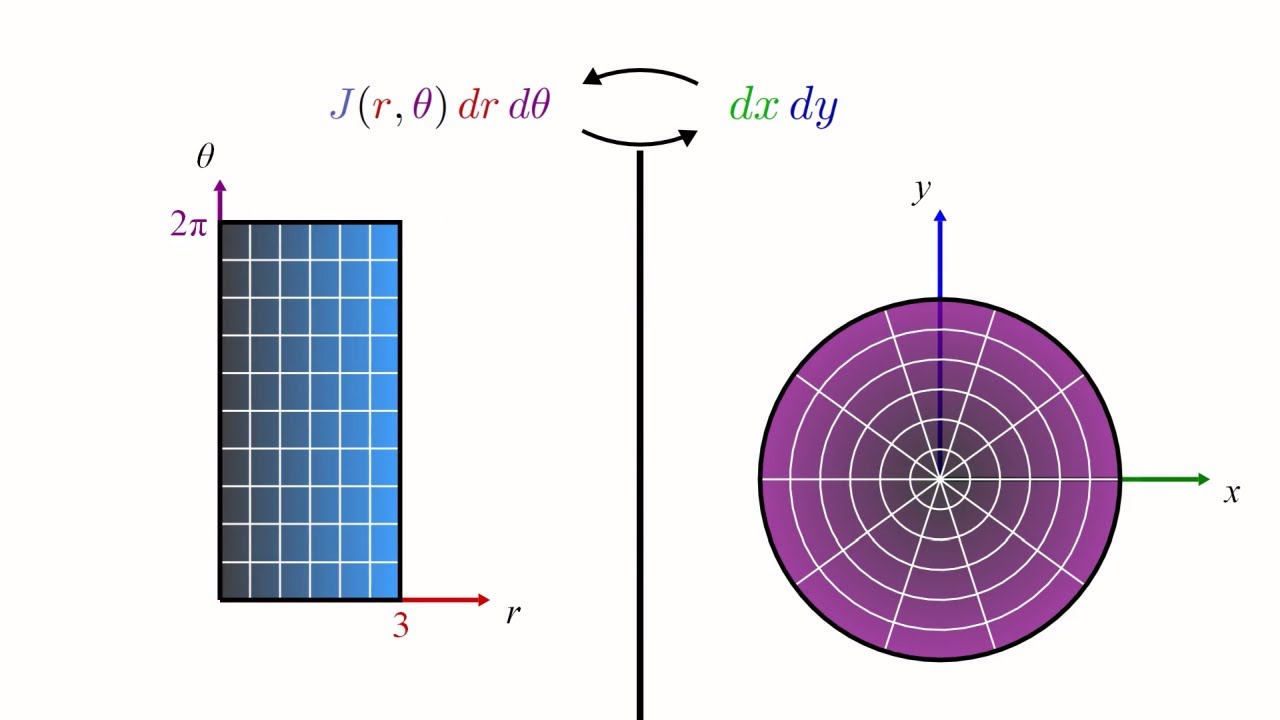
\includegraphics[width=0.5\linewidth]{LA Lecture notes/figures/polar vs descartes.jpg}
    \caption{Polar vs Descartes coordinates}
    \label{fig:enter-label}
\end{figure}

\section{The Hessian: Looking at Curvature}
Let's go back to a single scalar function $f(x, y, ...)$. We know the gradient $\nabla f$ involves first partial derivatives. What about \emph{second} partial derivatives?

We can take partial derivatives of the partial derivatives! For $f(x, y)$, we can compute:
\begin{align*}
    \frac{\partial}{\partial x} \left( \frac{\partial f}{\partial x} \right) &= \frac{\partial^2 f}{\partial x^2} \\\frac{\partial}{\partial y} \left( \frac{\partial f}{\partial x} \right) &= \frac{\partial^2 f}{\partial y \partial x}\\
    \frac{\partial}{\partial x} \left( \frac{\partial f}{\partial y} \right) &= \frac{\partial^2 f}{\partial x \partial y}\\
    \frac{\partial}{\partial y} \left( \frac{\partial f}{\partial y} \right) &= \frac{\partial^2 f}{\partial y^2}
\end{align*}

 For most nice functions you'll meet, the mixed partials are equal: $\frac{\partial^2 f}{\partial y \partial x} = \frac{\partial^2 f}{\partial x \partial y}$.

We can arrange these second partial derivatives into a matrix called the \textbf{Hessian matrix}, usually denoted by $H$:
$$ H = \begin{pmatrix} \frac{\partial^2 f}{\partial x^2} & \frac{\partial^2 f}{\partial x \partial y} \\ \frac{\partial^2 f}{\partial y \partial x} & \frac{\partial^2 f}{\partial y^2} \end{pmatrix} $$
For more variables, it just gets bigger, but always is a square matrix.

\textbf{What's the Hessian for?} Remember the second derivative test in single-variable calculus? $f''(x)$ told you about the concavity (whether the graph is bending upwards or downwards) and helped you classify critical points (local max, min, or neither).

The Hessian matrix does the same job in multiple dimensions! By looking at the properties of the Hessian matrix (like its eigenvalues or determinant) at a point where the gradient is zero ($\nabla f = \mathbf{0}$), we can figure out if that point is a:
\begin{itemize}
    \item Local minimum (like the bottom of a bowl)
    \item Local maximum (like the top of a hill)
    \item Saddle point (like the middle of a bimbim – curved up one way, down another)
\end{itemize}
So, the Hessian tells us about the "curvature" of the function's graph (which is a surface, or hypersurface, in higher dimensions).

?? Gradient descent \& backpropagation: refer to ML lectures




\end{document}